\chapter{Deployment}

\label{chap:deployment}

This chapter describes how to set up and deploy the application in a production environment. We look at using Docker to host the application in a container for reproducible deployment, setting up MySQL as the database for the application, and using Github Actions for continuous integration and deployment as the application is developed further.

\section{Docker}

\label{sec:docker}

With Docker, we can run the application inside a container. A container is an isolated sandbox process on the host system that runs an image that provides a file system and other OS properties for the application to run. This allows a container to be moved, stopped, started, deleted or created \cite{docker}. The image is defined in the Docker file on the root of the project and can then be used with ease on your own host system. 

\begin{minted}[frame=lines,framesep=2mm,baselinestretch=1.2,fontsize=\footnotesize,bgcolor=LightGray]{docker}
FROM gradle:7.6.1-jdk17 as Builder

# Add backend sources
WORKDIR /src
RUN mkdir api
ADD . /src/api
ADD start.sh /src/api/run/start.sh

# Build jar
WORKDIR /src/api
RUN chmod u+x gradlew
RUN ./gradlew build --exclude-task test

# Prepare runtime
FROM openjdk:17-alpine

WORKDIR /run/
COPY --from=Builder /src/api/API/build/libs/*-all.jar /run/api.jar
COPY --from=Builder /src/api/run/start.sh /run/start.sh

EXPOSE 80

RUN chmod +x /run/start.sh

ENTRYPOINT ["/run/start.sh"]
\end{minted}

The docker image is also hosted on the official docker hub, so the docker command can automatically download the image from the docker hub. 

With docker compose, an extension of docker, we can more easily define volumes, prots or other metadata for the application inside a docker container. This compose file could look like:

\begin{minted}[frame=lines,framesep=2mm,baselinestretch=1.2,fontsize=\footnotesize,bgcolor=LightGray]{yaml}
version: '3.8'
services:
  recommender:
    image: 12build/bpmn_recommender:latest
    restart: always
    volumes:
      - ./config.yaml:/etc/configs/config.yaml
\end{minted}

\section{MySQL}

\label{sec:sql}

MySQL is an SQL (Structured Query Language) database developed by Oracle \cite{MySQL}. We use this database for no particular reason over any other SQL database. MySQL is a relational database and is used to store user data, item data and user ratings. MySQL can be set up similarly to the application using the official docker image.

\begin{minted}[frame=lines,framesep=2mm,baselinestretch=1.2,fontsize=\footnotesize,bgcolor=LightGray]{yaml}
version: '3.8'
services:
  recommender:
    image: 12build/bpmn_recommender:latest
    restart: always
    volumes:
      - ./config.yaml:/etc/configs/config.yaml
    depends_on:
      - database
  database:
    container_name: DB
    image: mysql:latest
    environment:
      MYSQL_ROOT_PASSWORD: ${MYSQL_ROOT_PASSWORD}
      MYSQL_DATABASE: api
      MYSQL_USER: api
      MYSQL_PASSWORD: ${MYSQL_API_PASSWORD}
    ports:
      - "3306:3306"
    volumes:
      - ./db_data:/var/lib/mysql
\end{minted}

Before starting the application for the first time, all tables have to be created within MySQL, this can be done as shown in Appendix \ref{code:sql_tables} and the tables can additionally be filled with dummy data.

\section{Github Actions}

\label{sec:github_actions}

The application is being developed on Github, using Github Actions for automated testing and deployment. Github Actions is a tool within Github to manage CI/CD or Continuous Integration and Deployment. We use it to build and test the application when pushing new code into the repository, and to deploy to the Docker Hub when a new release is created.

\begin{figure}[h!]
\centering
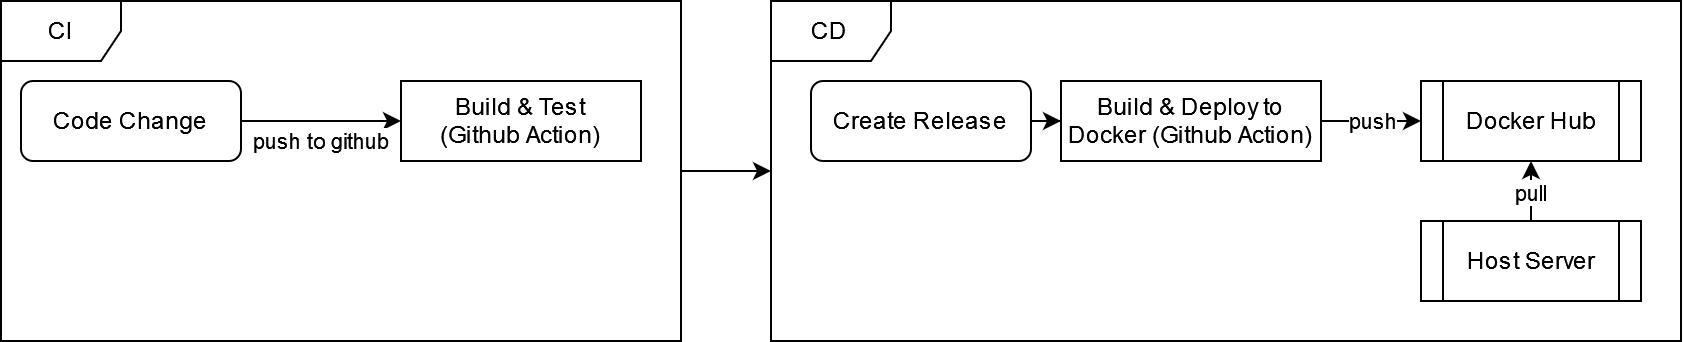
\includegraphics[width=\textwidth]{images/CICD_flow.drawio.png}
\caption{\label{fig:cicd}CI/CD Procedure}
\end{figure}


We define the build and test action shown in the Appendix \ref{code:github_build_and_test} and the deployment to the Docker Hub in the Appendix \ref{code:github_deploy}.